\documentclass[a4paper,12pt]{report}
\usepackage[spanish,activeacute]{babel}
\usepackage[utf8]{inputenc}
\usepackage{graphicx}
\usepackage{eurosym}
\usepackage{url}
\renewcommand\thesection{\arabic{section}}


\usepackage[T1]{fontenc}
\usepackage{times}
\usepackage[toc,page]{appendix}

\usepackage[strict]{changepage}
\usepackage{framed}


\usepackage{verbatim} % comentarios

\usepackage{xcolor}
\usepackage{color}
\definecolor{gray97}{gray}{.97}
\definecolor{gray75}{gray}{.75}
\definecolor{gray45}{gray}{.45}

\definecolor{darkblue}{rgb}{0.0, 0.0, 0.55}
\definecolor{formalshade}{rgb}{0.95,0.95,1}

\usepackage{listings}
\lstset{ frame=Ltb,
	framerule=0pt,
	aboveskip=0.5cm,
	framextopmargin=3pt,
	framexbottommargin=3pt,
	framexleftmargin=0.4cm,
	framesep=0pt,
	rulesep=.4pt,
	backgroundcolor=\color{gray97},
	rulesepcolor=\color{black},
	%
	stringstyle=\ttfamily,
	showstringspaces = false,
	basicstyle=\small\ttfamily,
	commentstyle=\color{gray45},
	keywordstyle=\bfseries,
	%
	numbers=left,
	numbersep=15pt,
	numberstyle=\tiny,
	numberfirstline = false,
	breaklines=true,
}

% minimizar fragmentado de listados
\lstnewenvironment{listing}[1][]
{\lstset{#1}\pagebreak[0]}{\pagebreak[0]}

\lstdefinestyle{consola}
{basicstyle=\scriptsize\bf\ttfamily,
	backgroundcolor=\color{gray75},
}

\lstdefinestyle{C}
{language=C,
}


\newenvironment{formal}{%
	\def\FrameCommand{%
		\hspace{1pt}%
		{\color{darkblue}\vrule width 2pt}%
		{\color{formalshade}\vrule width 4pt}%
		\colorbox{formalshade}%
	}%
	\MakeFramed{\advance\hsize-\width\FrameRestore}%
	\noindent\hspace{-4.55pt}% disable indenting first paragraph
	\begin{adjustwidth}{}{7pt}%
		\vspace{2pt}\vspace{2pt}%
	}
	{%
		\vspace{2pt}\end{adjustwidth}\endMakeFramed%
}


\begin{document}
	
	\pagestyle{empty}
	\begin{titlepage}
		\begin{center}
			
\includegraphics[scale=0.15]{images/fic01.png} \\ 
			\vspace{2cm} 
\includegraphics[scale=.4]{images/udc.pdf} \\
			
			
			\vspace{2.5cm}
			
			\textbf{\Large Diseño Software de Quake III Arena}\\
			\vspace{0.5cm}
			\large{Máster Universitario en Ingeniería Informática}\\
		\end{center}
		
		\vspace{7.2cm}
		\begin{flushright}
			\noindent Elena M. Delamano Freije
			
			\noindent Martín Álvarez Castillo
			
		\end{flushright}
	\end{titlepage}
	\clearpage
	
	
	\tableofcontents
	\clearpage
	
	
	\section{Introducción}
	Quake III Arena, a partir de ahora referido como \textbf{Q3}, es un videojuego de disparos en primera persona (\textit{FPS}) que fue lanzado en el año 1999 por \textit{id Software}. Este anticipado lanzamiento, al igual que el resto de juegos de \textit{id}, revolucionó el género de los FPS, tanto a nivel de diseño \,---\,el cual no se comentará en este documento, excepto donde sea relevante\,---\,, como a nivel de tecnologías e implementación de motor gráfico de tiempo real en el ámbito de los videojuegos. \cite{quake3}\\
	
	El nuevo motor desarrollado para crear Q3 fue bautizado como \textit{id tech 3}. Cuando existan referencias a Q3 en esta memoria, realmente se estará haciendo referencia a la versión de \textit{id tech 3} empleada para el desarrollo de Q3. Para desarrollos comerciales, \textit{id Software} ofreció una licencia de su nuevo motor a empresas de terceros. Una de las múltiples empresas que licenció \textit{id tech 3} fue Activision, para el desarrollo de la primera edición de \textit{Call of Duty}. La licencia del motor permitía la modificación del mismo y, a día de hoy, la familia de juegos de la franquicia de \textit{Call of Duty} todos usan una versión modificada cuya raíz es \textit{id tech 3}. \cite{idtech3}\\
	
	Asimismo, siguiendo la filosofía de ``compartir y colaborar para avanzar la tecnología'' del programador líder John Carmack, \textit{id Software} liberó todo el código fuente de Q3 bajo la licencia GPL-2.0 \cite{sourcecode}. La liberación de este código provocó que el juego fuera portado a muchas nuevas arquitecturas y, al tener dependencias con licencias abiertas, permitió que los seguidores hicieran versiones mejoradas del juego completamente retrocompatibles con el contenido pasado, añadiendo funcionalidades nuevas y arreglando bugs conocidos. Una de estas implementaciones de software libre muy popular es \textit{ioquake3} \cite{ioquake3}. \\
	
	Durante el desarrollo de este informe se utilizará el código inicialmente liberado en 2005, con una \textit{release} única, ya que no se ha subido un histórico de \textit{commits}, y cuyos programadores  \,---\, de acuerdo a los créditos \,---\, son John Carmack (director técnico y autor de la mayor parte del código), Robert A. Duffy y Jim Dose.\\
	
	El estado actual del proyecto es el mismo que cuando se desplegó la versión final del juego en 1999 (el código liberado en 2005 compila una versión exacta a la última versión disponible de Q3 en el momento). Aunque existen clones de este proyecto cuyo código ha sido limpiado sin introducir nuevos cambios o arreglar errores, se estudiará el código tal y como fue subido.\\
	
	
	\section{Metodología de Desarrollo y Herramientas}
	A diferencia del código principal del juego, las herramientas usadas para el desarrollo de Q3 nunca fueron liberadas. En esta época era muy habitual programar herramientas a medida para los desarrollos de tu motor (debugging, creación de mapas, importación y exportación de modelos, etc.). El juego final, al igual que sus predecesores, era muy fácil de modificar, los \textit{assets} del juego estaban claramente separados del código ejecutable y era posible cargar tus propios ficheros con modificaciones de cualquier tipo. El afán de crear este contenido hizo que aparecieran herramientas hechas por la comunidad que sustituían aquellas creadas internamente para el desarrollo, muchas de ellas son proyectos software libre de una complejidad bastante alta.\\
	
	\textit{id software} fue fundado por cuatro personas, y sus equipos de trabajo siempre fueron de tamaño reducido, dada la actitud vanguardista constante de la compañía las metodologías usadas no se basaban en nada existente, sino que fueron buscando sus propios principios y metodología a medida que realizaban proyectos, deshechando aquellos que no funcionaban para ellos.\\
	
	En una charla reciente de uno de los fundadores de \textit{id software}, John Romero, se detallan los principios que fueron descubriendo e integrando en su metodología de trabajo mediante una serie de citas, incluyendo el desarrollo de Q3. La mayoría de estos principios fueron consolidados antes del desarrollo de Q3, pero todos ellos seguían siendo la guía para el desarrollo de videojuegos en el proyecto de Q3. Analizamos y comentamos las citas a continuación:\\
	
	\begin{formal}
		\textit{No prototypes. Just make the game. Polish as you go. Don't depend on polish happening later. Always mantain constantly shippable code}
	\end{formal}
	El primer principio en el que se basaron los fundadores para competir en el mercado de los videojuegos con un equipo tan pequeño. Cada iteración del código apuntaba hacia la dirección del código entregable, es decir, cualquier parte desarrollada debía tener la complejidad suficiente para ser incluída en un producto entregable.
	
	\begin{formal}
		\textit{ It's incredibly important that your game can always be run by your team. Bulletproof your engine by providing defaults upon load failure.}
	\end{formal}
	Todos los juegos clásicos de \textit{id software} se regían por este principio, configuraciones específicas nunca deberían ser obligatorias. Si uno ejecuta Q3 (O cualquier juego clásico de \textit{id}) y pulsas enter en todos los menús (y ninguna tecla más) eres puesto en una partida contra la máquina con valores por defecto, sin necesidad de configurar nada.
	
	\begin{formal}
		\textit{Keep your code absolutely simple. Keep looking at your functions and figure out how you can simplify further.}
	\end{formal}
	Uno de los principios más revolucionarios para la época (1989), refactorizar código con el objetivo de constantemente simplificar y alcanzar un rendimiento mayor, ofreciendo una experiencia superior a la ofrecida por otros equipos más conformistas.
	
	\begin{formal}
		\textit{Great tools help make great games. Spend as much time on tools as possible.}      
	\end{formal}
	Desde muy pronto identificaron la necesidad de que todos los usuarios implicados en el proceso de desarrollo tuvieran herramientas que facilitasen su trabajo; los creadores de niveles tenían QuakeEd, un editor de mapas muy complejo. Los artistas disponían de herramientas para facilitar el flujo de trabajo en texturas y modelos, y los desarrolladores tenían entornos de pruebas y herramientas de debugging muy avanzadas (demo playback, virtual machines).\\
	El diseño del software se vio afectado por este principio, siempre desarrollando las tecnologías con la necesidad de poder utilizar potentes y flexibles herramientas para generar contenido o acelerar el desarrollo.
	
	\begin{formal}
		\textit{We are our own best testing team and should never allow anyone else to experience bugs or see the game crash. Don't waste other's time. Test thoroughly before checking in your code.}        
	\end{formal}
	Aunque hoy en día existen departamentos enteros de QA, era normal que los propios desarrolladores realizasen todas las pruebas sobre sus sistemas. Aún así, podemos identificar una versión primitiva de lo que actualmente son los \textit{pull request} y revisión de código, ya que el principio animaba a los desarrolladores a sólo entregar versiones bien probadas para integrar con el resto del equipo.
	
	\begin{formal}
		\textit{As soon as you see a bug, you fix it. Do not continue on. If you don't fix your bugs your new code will be built on a buggy codebase and ensure an unstable foundation.}        
	\end{formal}
	Una extensión del anterior principio, nunca entregar código en el que somos conscientes que hay errores, ya que estos pueden confundirse por decisiones de diseño deliberadas, y acumular errores en el diseño general.
	
	\begin{formal}
		\textit{Use a development system that is superior to your target.}       
	\end{formal}
	En 1993, durante el desarrollo de Doom, se decidió utilizar equipos de trabajo distintos a los equipos de prueba. Esto es una práctica muy común a día de hoy, pero en su momento era normal desarrollar con sistemas con la misma potencia disponible por los consumidores del software. Dar el salto a sistemas más potentes permitió acelerar los procesos de desarrollo y programar herramientas más ambiciosas.
	
	\begin{formal}
		\textit{Write your code for this game only - not for a future game. You're going to be writing new code later because you'll be smarter.}        
	\end{formal}
	Similar al principio de escribir código para el presente característico de XP. Es preferible resolver los problemas actuales en lugar de pensar en otros que aún no han surgido.
	
	\begin{formal}
		\textit{Try to code transparently. Tell your lead and peers exactly how you are going to solve your current task and get feedback and advice. Do not treat game programming like each coder is a black box. The project could go off the rails and cause delays.}        
	\end{formal}
	Desde el principio en \textit{id software} se trabajó con un ambiente colaborativo, muy distinto al habitual paradigma de tener desarrolladores completamente independientes trabajando solos en proyectos completos. Saber en qué punto del proyecto están tus compañeros ayuda a identificar bloqueos y problemas mucho antes de la fecha límite.\\
	
	\begin{formal}
		\textit{Programming is a creative art form based in logic. Every programmer is different and will code differently. It's the output that matters.}
	\end{formal}
	Soportar diferentes estilos de programación sólo funciona en equipos muy reducidos como este caso, pero es un principio poco recomendable cuando un proyecto tiene una duración más larga o un equipo más grande. \\
	\\
	En definitiva, podemos concluir que la metodología utilizada era una versión primitiva, casera e improvisada de Extreme Programming, muchos de los fundamentales aspectos de XP se ven reflejados en la filosofía de \textit{id software}. Probablemente podrían haber integrado con facilidad algunas técnicas modernas como programación por parejas y revisiones de código, así como control de versiones, con el fin de mejorar sus procesos de desarrollo.
	
	
	\section{Arquitectura de Software: Patrones y Antipatrones}

	La gran mayoría de aplicaciones están basadas en sistemas 2D que sólo requieren actualizar partes de la vista en cada momento. Cuando nos referimos a aplicaciones 3D, estas arquitecturas clásicas no son compatibles ya que, para dar sensación de fluidez y continuidad, el software debe generar una serie de frames cada segundo de manera constante. Incluso cuando el software no está haciendo ningún input, se produce el output de los frames. \\
	
	La arquitectura común de todos los aplicativos 3D es el render-loop:
	
	\begin{lstlisting}[style=C, numbers=none]
while (!quit)
{
	// Update the camera transform based on interactive
	// inputs (If real time) or by following a predefined path.
	updateCamera();
	// Update positions, orientations and any other
	// relevant visual state of any dynamic elements
	// in the scene.
	updateSceneElements();
	// Render a still frame into an off-screen frame
	// buffer known as the "back buffer".
	renderScene();
	// Swap the back buffer with the front buffer, making
	// the most recently rendered image visible
	// on-screen. (Or, in windowed mode, copy (blit) the
	// back buffer's contents to the front buffer.
	swapBuffers();
}
\end{lstlisting}
	
	
	En un videojuego, además de hacer el renderizado, se debe tener en cuenta la interactividad con el usuario, que en este caso afectará a muchos más elementos que el movimiento de la cámara. %, ya que el jugador afecta a%
	Para ello se introduce el concepto del \textit{game-loop}, un bucle que además de ejecutar las tareas de renderizado contiene toda la lógica de control del juego.\\
	
	 Un ejemplo básico de un game-loop sería el caso del videojuego clásico Pong:
	

	
		\begin{lstlisting}[style=C, numbers=none]
void main() // Pong
{
	initGame();
		
	while (true) // game loop
	{
	readHumanInterfaceDevices();
	if (quitButtonPressed())
	{
		break; // exit the game loop
	}
	movePaddles();
	moveBall();
	collideAndBounceBall();
	if (ballImpactedSide(LEFT_PLAYER))
	{
		incremenentScore(RIGHT_PLAYER);
		resetBall();
	}
	else if (ballImpactedSide(RIGHT_PLAYER))
	{
		incrementScore(LEFT_PLAYER);
		resetBall();
	}
	renderPlayfield();
	}
}
	\end{lstlisting}
	
	Esta aproximación de game-loop es demasiado básica y limitada para juegos modernos. Aún así, la arquitectura de dichos juegos se basa un game-loop que contiene a su vez una serie de bucles de cada subsistema del motor, pudiendo correr cada uno de esos bucles a un frecuencia distinta del resto. Por ejemplo: en un segundo queremos renderizar 60 fotogramas, pero sólo tenemos que recibir paquetes de red 30 veces por segundo. 
	
	Se destacan dos aproximaciones muy frecuentes en el desarrollo de motores de videojuegos:
	
	\begin{itemize}
		\item \textbf{\textit{Callback-Driven frameworks}}. La mayoría de los subsistemas de motores y de paquetes middleware de videojuegos están estructurados como librerías. Para la implementación del game-loop se usan las llamadas a esos subsistemas a partir de sus API's para agilizar la lógica de cada subsistema en cada iteración. Por ejemplo: si se estuviera implementando el juego de \textit{Flappy bird} utilizando este estilo, una iteración del bucle podía parecerse a algo similar a:
		
		\begin{lstlisting}[style=C, numbers=none]
void main() // Flappy Bird
{
  GameLogic.initGame();
  Audio.playBackgroundMusic();
  while (true) // game loop
  {
    Input.readHumanInterfaceDevices();
    if (input.screeenTouched())
    {
      Physics.increaseBirdUpMomentum(); // exit the game loop
    }
    GameLogic.moveBird();
    GameLogic.scrollScreen();
    if (Physics.birdCollision() //If the bird collides with ground or pipe
    {
      break; //Exit game loop
    }
    Audio.playSoundEffects();
    Graphics.renderScreen();
  }
  Networking.loadHighScores(); //
  GameLogic.playGameOverScreen();
}
		\end{lstlisting}
		
		
		El programador, en este ejemplo, sólo ha tenido que diseñar la lógica de cómo funciona el juego y ha dejado en manos de los subsistemas la ejecución de bajo nivel de los resultados de la interacción del usuario. Los subsistemas utilizados en este caso, y de los que el programador no está obligado a conocer más que sus API's, serían las implementaciones de networking, de audio, de gráficos, de input y de físicas. La mayoría de estas librerías son independientes e intercambiables entre sí, a las que se accede utilizando un patrón facade.
		
		Si en el futuro el programador decidiera programar este juego para iOS, este código tendría que adaptar las llamadas de API a las librerías disponibles en iOS, quizá utilizando el \textit{\textbf{patrón adaptador}} para evitar cambiar la lógica principal y los tipos de datos de su sistema.	
		
		\item \textit{\textbf{Event-Based Updating}}. En este estilo de implementación todos los subsistemas son capaces de enviar y recibir eventos. Estos eventos son similares a los que se usan en los patrones de interfaces gráficas como MVC. 
		
		En el game-loop se han de procesar todos los eventos recibidos en la anterior iteración y distribuirlos a los subsistemas pertinentes para que los procesen. Además, también se debe de encargar de notificar a los subsistemas de en qué instante se encuentra la ejecución del programa. Los eventos recibidos no siempre tienen por qué ser procesados inmediatamente, por lo que cada subsistema debe de tener capacidad para almacenar eventos y en base a la información del bucle principal, ser consciente del instante en el que ha de procesar cada uno de los eventos. 
		
		La implementación de este modelo puede ser completa, separando todos los subsistemas, o usarse sólo para ciertos subsistemas, como suele ocurrir en motores en los que se implementó \textit{a posteriori} y en los que era muy difícil desacoplar el subsistema de rendering de otros que dependían de él como: físicas, audio e IA.
	
	    A lo largo de este trabajo se comentarán patrones apoyados en esta arquitectura basada en eventos.
		
	\end{itemize}	

%INTRODUCRIR BIBLIOGRAFIA LIBRO%	
	
	El motor \textit{id tech 3} y sus antecesores utilizan una arquitectura completamente basada en eventos que desacopla los ciclos de vida de los diferentes subsistemas del motor. Una buena aproximación para entender la arquitectura es representar como una caja negra el sistema (\textit{Quake3.exe}). Como se puede ver en la Figura \ref{figarchitectureblackbox}, el software sólo recibe entradas de red y teclado/ratón, y produce salidas de red y de frames.
	
	
	\begin{center}
		\begin{figure}[h]
			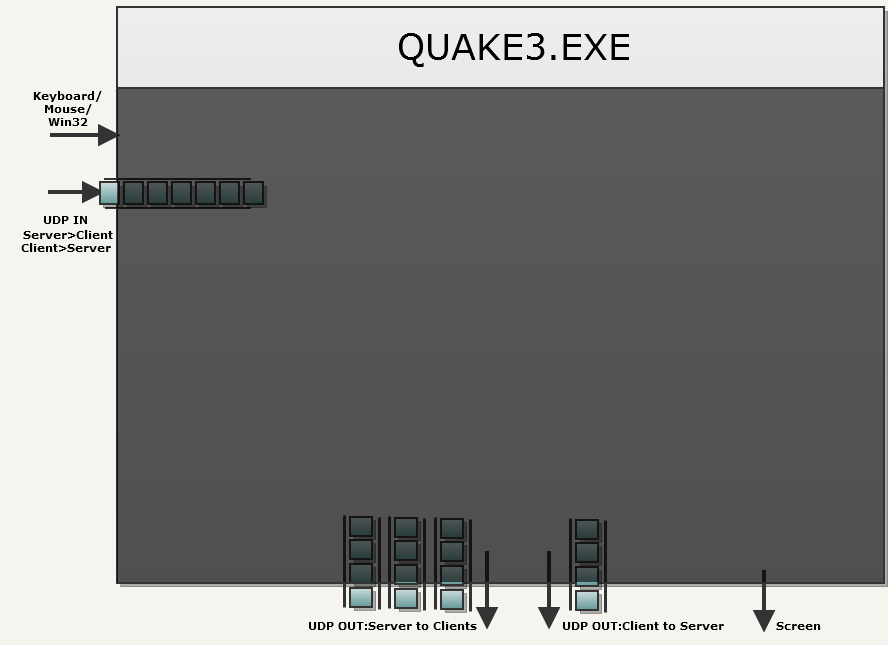
\includegraphics[width=1\textwidth]{images/q3_architecture_blackbox}
			\caption{Q3 architecture blackbox}
			\label{figarchitectureblackbox}
		\end{figure}
	\end{center}

	Dentro del sistema se identifican 6 módulos: aplicación principal y lógica de juego (\textit{quake3.exe}), rendering (\textit{renderer.lib}), IA (\textit{bot.lib}), lógica servidora (\textit{game}), lógica cliente (\textit{cgame}) e interfaz de usuario (\textit{q3\_ui}), representados en la Figura 2 \begin{comment}\ref{fig:architecture}\end{comment} 

		\begin{center}
			\begin{figure}[h]
				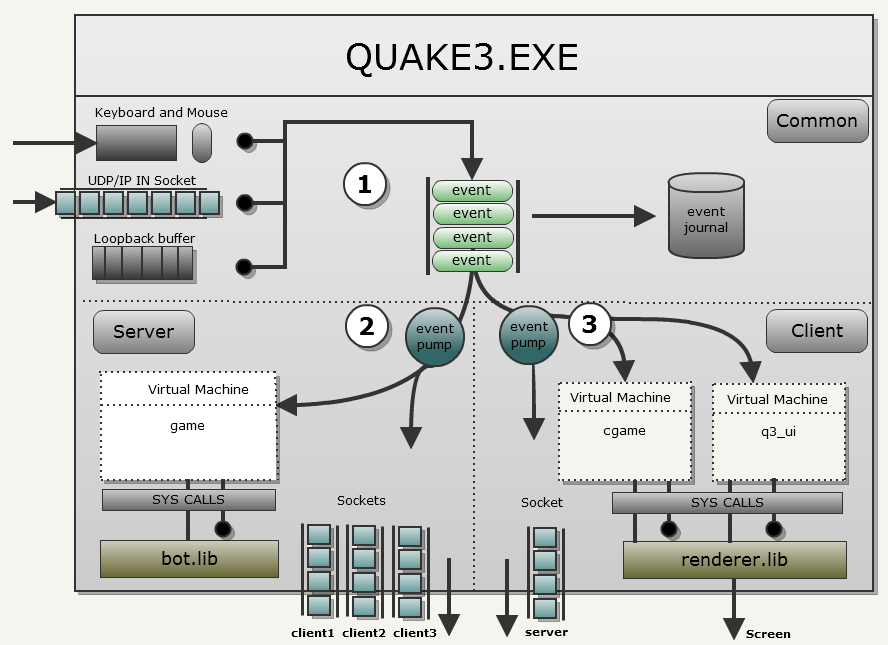
\includegraphics[width=1\textwidth]{images/q3_architecture}
				\caption{Q3 architecture}
				\label{figarchitecture}
			\end{figure}
		\end{center}
	
	En esta arquitectura se destacan dos decisiones de diseño muy importantes:
	
	\subsubsection{Bitácora de inputs para facilitar las pruebas}
	
	Cada uno de los inputs recibidos (Teclado, mensaje win32, ratón, socket UDP) es convertido a \textit{event\_t} y encolado en una cola de eventos (\textit{sysEvent\_t eventQue[256]}). Con esta aproximación se puede mantener una bitácora de estos inputs que, junto con otros factores también almacenados, permiten ser reproducidos en orden para recrear bugs de manera consistente. \cite{johncplan}\\
	
	En la figura \ref{figarchitecture} se identifican dentro de la parte \textit{Common} el administrador de inputs, la cola de eventos y el \textit{event journal} mencionado.
	
	\subsubsection{Separación explícita de cliente y servidor}
	
	Durante el desarrollo de \textit{id tech 3} se decidió tomar la decisión de implementar una arquitectura cliente-servidor en la que los roles y subsistemas de cada uno de los dos fueran significativamente distintos. Hasta entonces los clientes y servidores contenían el mismo código pero debían desempeñar roles distintos.\\
	
	En Q3 el servidor es el responsable de mantener el estado de la partida, determinar información de la partida necesitan los clientes y propagarla por la red. Se puede observar en la imagen que \textit{bot.lib} está contenido únicamente dentro de la parte servidora, ya que es también la encargada de proveer la lógica e inputs de los jugadores controlados por la IA.\\
	
	El cliente es responsable de predecir dónde están los objetos en cada instante, incluyendo los elementos afectados por la red utilizando una técnica llamada \textit{lag compensation}, y de renderizar la vista para el usuario \,---\, De nuevo, en la figura  \ref{figarchitecture} se puede observar como\textit{ renderer.lib} está contenido en la parte cliente. \cite{architecture}\\
	
	\subsubsection{Eventos desde el punto de vista del código}
	
	Para ilustrar la producción/consumición de eventos se puede estudiar el bucle principal (\textit{main}) del código de Q3. Se muestra un ejemplo resumido (Código omitido y desenroscado):
	
	\begin{lstlisting}[style=C, numbers=none]
int WinMain(HINSTANCE hInstance, HINSTANCE hPrevInstance, LPSTR lpCmdLine, int nCmdShow)
{
  Com_Init
	
  NET_Init
	
  while( 1 )
  {
     // Codigo de Common 
    IN_Frame()  // Inyecta los inputs de Win32 joystick y raton en la cola unificada de eventos como event_t.
    {
      IN_JoyMove
      IN_ActivateMouse
      IN_MouseMove
    }
    
    Com_Frame
    {
      // Codigo de Common 
      Com_EventLoop // Envia mensajes win32, paquetes UDP del socket y comandos de la consola a la cola
      (sysEvent_t eventQue[256])
      Cbuf_Execute
      
      // Codigo de Servidor (SV)
      SV_Frame
      {
        SV_BotFrame // Llamada a bot.lib para avanzar su logica
        VM_Call( gvm, GAME_RUN_FRAME, svs.time ) // Llamada a la Game Virtual Machine para procesar la logica de juego
        SV_CheckTimeouts
        SV_SendClientMessages  // Enviar el snapshot o delta snapshot (diferencia entre el snapshot anterior y el actual) a los clientes conectados
      } 
      
      // Codigo de Common aqui
      Com_EventLoop
      Cbuf_Execute
      
      // Codigo de cliente (CL)
      CL_Frame
      {
        CL_SendCmd // Eenviar los comandos al servidor usando la cola de eventos.
        
        SCR_UpdateScreen
        VM_Call( cgvm, CG_DRAW_ACTIVE_FRAME); // Enviar mensajes a la Client Virtual Machine (encargada de hacer las predicciones).
        or
        VM_Call( uivm, UI_DRAW_CONNECT_SCREEN); // Envia un mensaje a la UI Virtual Machine si esta el menu abierto
        
        S_Update // Actualizar los buffers de sonido
      }
    }
  }
}
	\end{lstlisting}

    En este código se puede observar la potencia del patrón basado en máquinas virtuales, que permite obviar las llamadas de renderizado en el bucle principal del juego. Lo único que necesita hacer este bucle es enviar un mensaje (evento) a la máquina virtual del cliente (\textit{CG\_DRAW\_ACTIVE\_FRAME}) indicándole que es necesario realizar un refresco (cargar el siguiente fotograma).\\
    
    Esta máquina virtual realiza los trabajos de culling y predicción antes de llamar a las librerías de OpenGL usando una llamada del sistema Q3 (\textit{CG\_R\_RENDERSCENE}). Cuando Quake.exe recibe esta llamada es cuándo realmente se llama a la función de renderizado de la escena (\textit{RE\_RenderScene}).\cite{unrolled_loop_source}\cite{unrolled_loop}\\   
    
    \begin{center}
    	\begin{figure}[h]
    		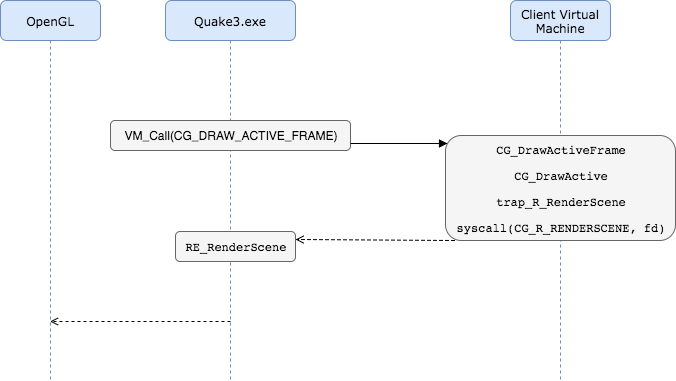
\includegraphics[width=1\textwidth]{images/diagrama.png}
    		\caption{Diagrama de flujo VM}
    		\label{figdiagrama}
    	\end{figure}
    \end{center}
    
    En la figura \ref{figdiagrama} se puede visualizar esta explicación. En lugar de tener todas las llamadas acopladas y dependientes del mismo ciclo de vida, se aprovecha la arquitectura de mensajes para que cada componente realice su trabajo cuando esté listo para procesarlo. Además, esto implica que Quake3.exe no tiene necesidad de saber qué trabajos va a realizar la \textit{Client Virtual Machine} antes de lanzar el mensaje para hacer el render de la escena.\\
    
    

  
	
	
	\newpage
	\section{Diseño de Software}
	

	
	El software de Quake III Arena está considerado un buen ejemplo de programación estructurada, que gira en torno a una adecuada definición de funciones y a un equilibrio respecto a la complejidad de las mismas. En la versión que se está analizando en esta memoria, se puede observar que el código está bien diseñado y estructurado, pudiendo tener una visión global de su estructura.\\
	
	El desarrollo ha sido realizado íntegramente utilizando el lenguaje C \,---\,es decir, un lenguaje no orientado a objetos \,---\, por lo que no se pueden encontrar patrones de diseño software tal y como se está acostumbrado a encontrarlos. Pero esto no implica que no puedan estar presentes a lo largo del código. Se ha intentado localizar algunos conocidos como el \textit{memento}, \textit{command} y \textit{interpreter}, y a continuación se expondrá la implementación concreta de ellos:\\
	
    \subsection{Memento Pattern: Arquitectura de Red basada en Snapshots}
	Para coordinar los estados de la partida en el servidor, con el fin de sincronizar todos los clientes y generar estados consistentes basándose en la interacción de los mismos, Q3 utiliza una implementación del \textit{patrón memento}.\\
	
	\begin{center}
		\begin{figure}[h]
			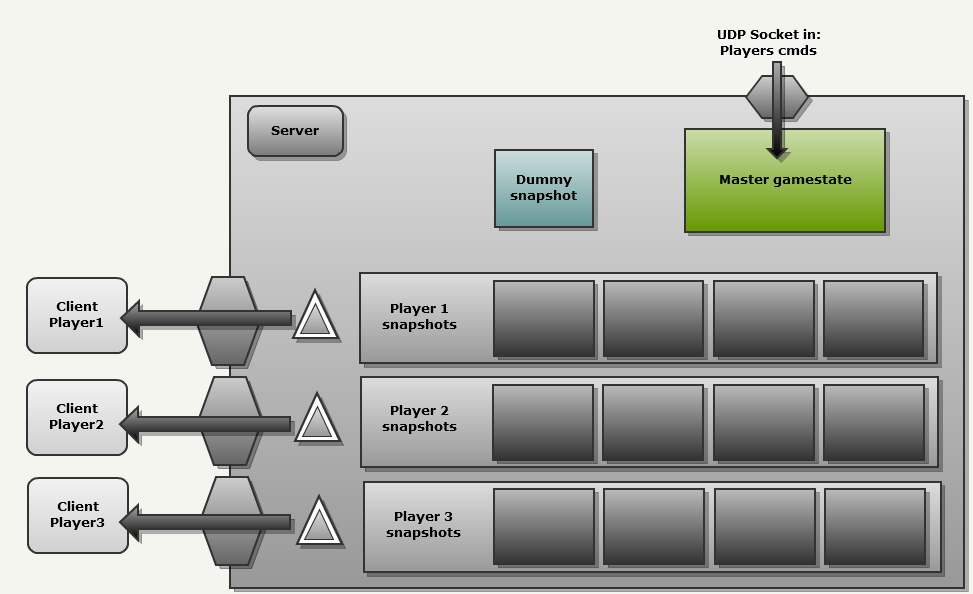
\includegraphics[width=1\textwidth]{images/q3_network_arch}
			\caption{Q3 architecture virtual machines}
			\label{figq3network}
		\end{figure}
	\end{center}

	Dentro del módulo servidor existe un denominado \textit{Master gamestate} que representa el estado veraz y universal de la partida. Cada cliente almacena los últimos 32 estados en un lista circular, estos estados son llamados \textit{snapshots}. El dummy snapshot es un estado con todos los valores a 0 utilizado para calcular el delta (diferencia entre el estado actual y el siguiente) cuando no existe estado anterior.\\
	
	Simplificando mucho el funcionamiento del networking, los clientes no envían y reciben estados completos, sino que guardan los últimos estados con el fin de sólo enviar y recibir la diferencia entre estados, omitiendo información repetida, sólo actualizando lo necesario. Si fuera necesario, se podría mandar el estado completo en lugar de una actualización parcial.\\
	
	La ventaja de esta implementación reside en la posibilidad de enviar la diferencia entre estados arbitrariamente antiguos. Es decir, si un cliente no recibió una actualización de un estado (por problemas de conectividad, por ejemplo), no es viable re-enviar la paquetería de ese estado y, de hecho, no sería posible ya que toda la paquetería de red en Q3 es basada en UDP. En su lugar, se ignora esa actualización y en la siguiente actualización el cliente reportará al servidor el estado de su mundo, el servidor simplemente manda la diferencia entre el estado maestro y su estado, sin importarle cuántos snapshots de retraso tenga el cliente (hasta el límite de snapshots) y sin necesidad de implementar control sobre los estados concretos. Si la diferencia es suficientemente grande, podría provocar un reenvío del estado completo.
	
	%Introducir algo de código de networking?

	\subsection{Command pattern: Quake Virtual Machines}
	
	Por motivos de rendimiento y portabilidad, la lógica del juego en Q3 (y antiguos Quakes) se ejecuta encapsulada en las llamadas Quake Virtual Machines, que son un sistema similar a un `Sandbox' que limita las instrucciones que se pueden utilizar y cómo se ejecutan. Su comportamiento es similar a la JVM respecto a que el código escrito para Q3VM corre en todos los sistemas que tengan Q3VM interpreter. \cite{q3vm}\\
	
	\begin{center}
		\begin{figure}[h]
			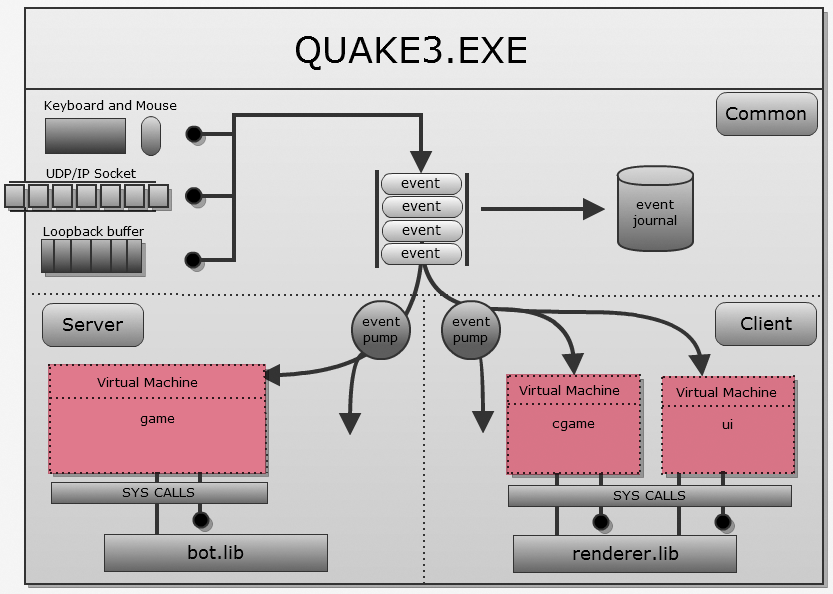
\includegraphics[width=1\textwidth]{images/q3_workspace_architecture}
			\caption{Q3 architecture virtual machines}
			\label{figq3vm}
		\end{figure}
	\end{center}
	
	Los módulos de \textit{game}, \textit{cgame} y \textit{q3\_ui} están escritos para Q3VM, y para acceder a ellos se ha de emplear la llamada de acceso \textit{VM\_Call( vm\_t *vm, int callnum, ... )}. Esta llamada es interpretada por la Q3VM, que extrae las instrucciones que debe ejecutar según los parámetros de la llamada. El cliente que realiza la llamada no tiene conocimiento del contenido de la operación a la que llama, pero usando la encapsulación en la VMCall puede hacer uso de la operación.\\
	
	El flujo de una VMCall sería así:
	
	\begin{itemize}  
		\item La VMCall se construye con hasta 11 parámetros, y escribe cada valor de 4 bytes en el bytecode de la VM (\textit{vm\_t *vm}) con valores desde 0x00 hasta 0x26
		\item La VMCall pasa el id del mensaje localizado en 0x2A
		\item El interpreter comienza a interpretar los opcodes empezando en 0x2D
		\item vmMain es el encargado de hacer dispatch y enrutado del mensaje al método correspondiente al bytecode
	\end{itemize}

	\begin{center}
		\begin{figure}[h]
			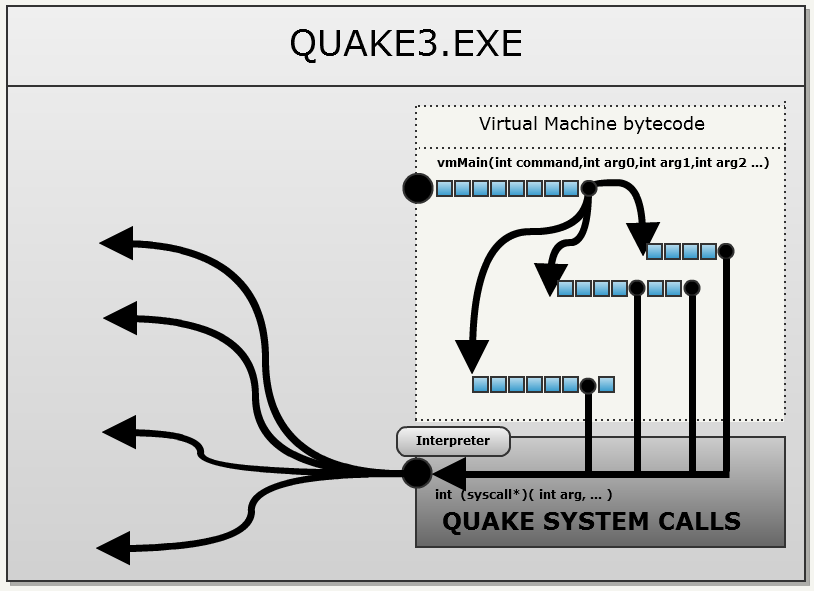
\includegraphics[width=1\textwidth]{images/vm_bb}
			\label{fig:q3vm_bb}
			\caption{Q3 virtual machine Bytecode interpreter}
		\end{figure}
	\end{center}

	Un ejemplo concreto de esto podemos observarlo en el \textit{main} del código servidor:
	
		\begin{lstlisting}[style=C, numbers=none]
// run the game simulation in chunks
while ( sv.timeResidual >= frameMsec ) {
	sv.timeResidual -= frameMsec;
	svs.time += frameMsec;
	
	// let everything in the world think and move
	VM_Call( gvm, GAME_RUN_FRAME, svs.time );
}
	\end{lstlisting}
	
	Tras realizar sus tareas previas, el servidor pasa el control a \textit{game} mediante una llamada a su VM, pasándole el parámetro \textit{GAME\_RUN\_FRAME} que indica al módulo \textit{game} que tiene que hacer los cálculos necesarios para procesar el siguiente frame basándose en la referencia de tiempo. El código del servidor está completamente abstraído de los cálculos para generar el siguiente frame.\\
	 \cite{q3vmcallex}

	Para la comunicación en el sentido opuesto, la Q3VM utiliza llamadas del sistema para comunicarse con Quake3. Estas llamadas del sistema están definidas en los ficheros cabecera del \textit{Client VM}\cite{q3vmclient} y \textit{Server VM}\cite{q3vmserver}\\
	
	
	Además de utilizar este command pattern para ejecutar operaciones implementadas en código ejecutable por la Q3VM, las Q3VM también son capaces de ejecutar bytecode compilado en instrucciones x86 y código compilado para dll de Windows. \cite{q3vmbb}
	
	
		\subsection{Interpreter pattern: Quake Console}
	Una de las herramientas más potentes integradas en Q3 es la consola del desarrollador. Con ella el usuario puede introducir comandos para afectar a variables internas y configuraciones. Todas las operaciones de menús tienen un equivalente accesible por la consola, aunque su utilidad se extiende más allá, permitiendo incluso ser utilizada para mostrar mensajes informativos al usuario durante la partida de manera dinámica y estándar.\\
	
	Para conseguir esto se hace uso de un patrón interpreter para procesar el comando y sus parámetros, y convertirlos en las instrucciones a ejecutar para modificar las propiedades del motor pertinentes.\cite{console_source}\cite{consolecmd_source}\\
	
	Cuando el cliente escribe un comando en su consola local se ejecuta en \textit{cgame} la llamada para el intérprete de comandos utilizando una llamada del sistema (Q3VM -> Q3):\\
	
	\begin{lstlisting}[style=C, numbers=none]
void CG_TargetCommand_f( void ) {
int		targetNum;
char	test[4];

targetNum = CG_CrosshairPlayer();
if (!targetNum ) {
return;
}

trap_Argv( 1, test, 4 );
trap_SendConsoleCommand( va( "gc %i %i", targetNum, atoi( test ) ) );
}
	\end{lstlisting}
	
	
	
	
A pesar de que es un código que llama la atención por su buena estructura, también se debe de exponer que contiene algunos antipatrones en él.\\

Por ejemplo:\\

\subsection{Vendor Lock-in}

Se trata de un antipatrón de arquitectura, en el que se puede observar bloqueo por parte de proveedor. Esto ocurrenen sistemas que dependen, en gran medida, de arquitecturas propietarias.

Para el renderizado de los graficos en este sistema se ha utilizado OpenGL y, a pesar de que no está acoplado con el código, el motor depende de la existencia de la librería. En el caso de que un sistema no tenga soporte para OpenGL, habría que portar toda la capa de integración al correspondiente sistema de renderizado.  \\


\subsection{The blob}

Se trata de un antipatrón de diseño, en el que el diseño de estilo de procedimiento conduce a un objeto con la mayor parte de las responsabilidades, mientras que la mayoría de los demás objetos solo contienen datos o ejecutan procesos simples. La solución incluye la refacturación del diseño para distribuir las responsabilidades de manera más uniforme y aislar el efecto de los cambios.

El código de Q3 está separado en unidades funcionales, de manera que se evita crear ficheros o sistemas monolíticos como los que define este antipatrón.

Una excepción a estas buenas prácticas se puede ver en la parte de IA. Durante el desarrollo de Q3, el programador líder de \textit{id Software} delegó la tarea de desarrollar los \textit{bots} a un desarrollador de la compañía, que no consiguió entregar un trabajo finalizado. Los \textit{bots} no tenían el comportamiento esperado, si no que eran muy predecibles y con movimientos antinaturales. En un juego basado en partidas multijugador, esto era una parte importante. Para solucionar este bloqueo, \textit{id Software} decidió dejar este trabajo en manos de Jean-Paul van Waveren (a.k.a Mr.Elusive), que integró toda la librería de \textit{bots} en un sistema completamente separado y cerrado que se decidió colocar dentro de la arquitectura en la parte de servidor, pero fuera de la VM. Para comunicarse con el juego (VM) se usaron \textit{syscalls}. Esto es un claro ejemplo del antipatrón de \textit{The blob}, ya que toda esta lógica debería de estar integrada y repartida dentro las unidades funcionales del código de la VM.

	\begin{center}
	\begin{figure}[h]
		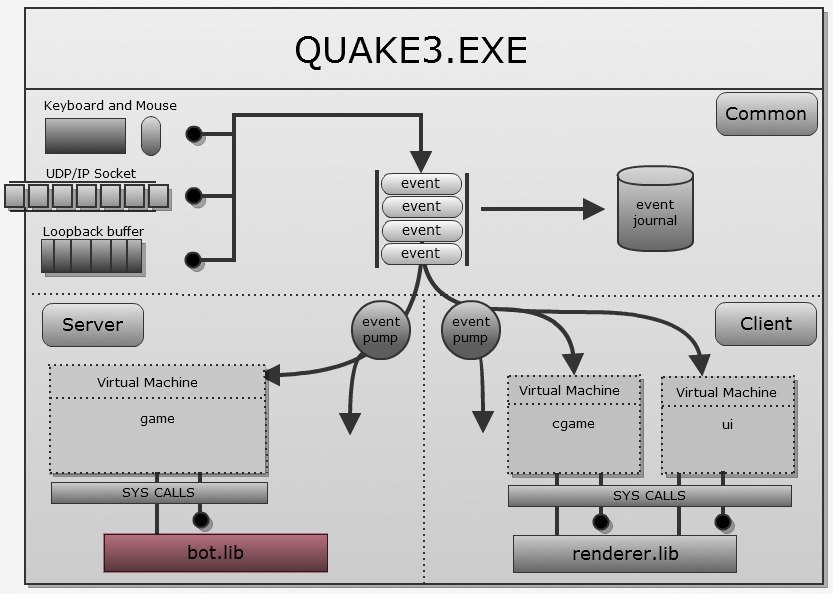
\includegraphics[width=1\textwidth]{images/bot}
		\label{fig:bot}
		\caption{Bot.lib}
	\end{figure}
\end{center}

A pesar de ser un antipatrón, el código está muy bien desarrollado dentro de su propio sistema y el creador hizo un artículo de investigación en el que entra en detalles sobre la implementación.\cite{quake3}\\


	
	\section{Calidad del Software}
    El software se distribuyó en una única release, ofreciendo el código fuente del motor y unas breves líneas de cómo compilar para Windows, Linux y Mac. No se proporciona más documentación que este breve \textit{README}, aunque la gente que ha trabajado con este código liberado dice no haber tenido problema para familiarizarse con el código usando los comentarios y la claridad del estilo utilizado, con ficheros y clases bien diferenciadas.\\
    
    No se acompaña el código, tampoco, con ningún tipo de test, por lo que cualquier modificación propia podría introducir cambios y regresiones en las features ya implementadas sin ningún tipo de manera de comprobarlo de manera automática. La filosofía en \textit{id software} estaba basada en que el testing era una tarea más del programador sobre su propio código, además de realizarlo mediante playtesting diario para comprobar la integración. Automatizar las tareas de testing para un videojuego online es difícil, de manera que actualmente se sigue empleando el testing via playtesting entre jugadores reales, pero sí se echan en falta \textit{unit tests} sobre módulos en los que podría encajar hacerlos.\\
    
    Respecto al performance en Q3, se incluyen varias herramientas\textit{ in-game }para medir todo tipo de parámetros relacionados. Se pueden distinguir entre dos grandes grupos: las mediciones sobre el performance gráfico (como los fotogramas por segundo y \textit{frame time}) y las mediciones sobre la red, accesibles mediante la variable \textit{CG\_LAGOMETER}. Con el Lag-o-Meter se pueden obtener gráficas sobre el estado de la conexión entre el cliente y el servidor, de esta manera podrían observarse cuellos de botella o problemas en los protocolos de red implementados.
	
	\section{Estado de la accesibilidad en el proyecto}
    Al ser un juego de acción rápida contra oponentes por Internet no existe ningún tipo de consideración para la accesibilidad de ningún tipo. Aún así, existen algunas features que se podrían haber incluído para mejorar la accesibilidad del software como: paletas de colores,  ajustes de brillo y contraste extremos para usuarios con problemas de visión, e indicadores visuales y subtítulos para usuarios con problemas auditivos.
	
	\section{Conclusiones}
	TODO\\
    
	
	\begin{thebibliography}{9}
		
		\bibitem{johnromeroyoutube}The Early Days of Id Software. \emph{John Romero}. URL: \url{https://www.youtube.com/watch?v=KFziBfvAFnM}\\
		\bibitem{quake3}Quake III Arena. \emph{Quake Wikia}. URL: \url{http://quake.wikia.com/wiki/Quake_III_Arena}\\
		\bibitem{idtech3} id tech 3. \emph{Giant Bomb}. URL: \url{https://www.giantbomb.com/id-tech-3/3015-1918/}\\
		\bibitem{sourcecode} Quake III Arena Source Code. \emph{Github}. URL: \url{https://github.com/id-Software/Quake-III-Arena}\\
		\bibitem{ioquake3} ioquake3. \emph{ioquake3}. URL: \url{https://ioquake3.org/}
        \bibitem{johncplan} John Carmack's 14 Oct 1998 .plan (Archived from original). \emph{John Carmack}. URL: \url{https://raw.githubusercontent.com/ESWAT/john-carmack-plan-archive/master/by_day/johnc_plan_19981014.txt}
		\bibitem{architecture} Quake 3 Source Code Review. \emph{Fabien Sanglard}. URL: \url{http://fabiensanglard.net/quake3/index.php}
		\bibitem{unrolled_loop_source} Quake 3 Main. \emph{id software}. URL: \url{https://raw.githubusercontent.com/id-Software/Quake-III-Arena/master/code/win32/win_main.c}
        \bibitem{unrolled_loop} Quake 3 Loop Unrolled. \emph{Fabien Sanglard}. URL: \url{http://fabiensanglard.net/quake3/q3_loop_unrolled.txt}
        \bibitem{q3vm} Quake 3 Virtual Machines. \emph{phaethon}. URL: \url{https://www.icculus.org/homepages/phaethon/q3mc/q3vm_specs.html}
        \bibitem{q3vmcallex} Quake 3 Server Main. \emph{id software}. URL: \url{https://raw.githubusercontent.com/id-Software/Quake-III-Arena/master/code/server/sv_main.c}
        \bibitem{q3vmclient} Quake 3 Client Main. \emph{id software}. URL: \url{https://raw.githubusercontent.com/id-Software/Quake-III-Arena/master/code/game/g_public.h}
        \bibitem{q3vmserver} Quake 3 Server VM. \emph{id software}. URL: \url{https://raw.githubusercontent.com/id-Software/Quake-III-Arena/master/code/cgame/cg_public.h}
        \bibitem{q3vmbb} Quake 3 Virtual Machine. \emph{Fabien Sanglard}. URL: \url{http://fabiensanglard.net/quake3/qvm.php}
		\bibitem{console_source} Quake 3 Console. \emph{id software}. URL: \url{https://raw.githubusercontent.com/id-Software/Quake-III-Arena/master/code/client/cl_console.c}
		\bibitem{consolecmd_source} Quake 3 Console Commands. \emph{id software}. URL: \url{https://raw.githubusercontent.com/id-Software/Quake-III-Arena/master/code/cgame/cg_consolecmds.c}	
		\bibitem{JeanPaulArticle} The Quake III Arena Bot. 28 Jun 2001. \emph{J.M.P. van Waveren}. URL: \url{The Quake III Arena Bot}		
	\end{thebibliography}


	
	
\end{document}
